\documentclass{article}
\usepackage{amsmath}
\usepackage{lmodern}
\usepackage[english]{babel}
\usepackage[utf8]{inputenc}
\usepackage[a4paper, margin=2.5cm]{geometry} 
\usepackage{titlesec}
\usepackage{enumitem} 
\usepackage{xcolor}
\usepackage{hyperref}
\usepackage{graphicx}
\usepackage{float}

\newcommand{\reqnum}[1]{\textbf{\underline{RF-#1}}}
\newcommand{\reqnumNF}[1]{\textbf{\underline{RNF-#1}}}



% Ajuste fino de listas
\setlist[itemize]{left=2.5em, labelsep=1em, itemsep=0.4em, topsep=0.6em}

\title{Workshop 2}
\author{
Henry Ricaurte Mora 20221020084 \\
Germán Darío Aya Fuentes 20232020091 \\
Javier Alejandro Penagos Hernández 20221020028
}
\date{}

\begin{document}

\maketitle

\section{Review Workshop {\#}1 Findings}

In Workshop \#1, a detailed analysis was conducted on the system behind a Kaggle competition focused on predicting student performance in a game-based learning environment. The primary objective of this system is to determine, based on behavioral data collected during interaction, whether a student will answer a question correctly. This prediction is directly related to the level the user reaches in the game, which reflects both skill and progress.

\subsection*{Key Findings}

\subsubsection*{System Components}

The analysis identified an architecture composed of multiple interconnected elements forming a complex cyber-physical system:

\begin{itemize}
    \item \textbf{Inputs}: User interaction begins with the \textit{mouse}, whose main events are \textit{hover} and \textit{click}. These are recorded with Cartesian coordinates (\textit{x, y}) and routed through the system.
    
    \item \textbf{Processing}: Events are handled by modules such as \textit{screen}, \textit{room}, and \textit{recept}, which interact with the \textit{event handler}. The \textit{event handler} assigns a \textit{name} and \textit{text} to each event and forwards them to the \textit{event registry}.
    
    \item \textbf{Identification and Context}: Each user is associated with a \textit{user id}, which relates to parameters such as \textit{level}, \textit{configuration} (fullscreen, music option, visual quality), and \textit{session id}.
    
    \item \textbf{Analytics}: All events are registered and processed by the \textit{data analytic} module, responsible for generating a prediction of the student’s \textit{performance}, i.e., their ability to correctly answer questions.
\end{itemize}

\subsubsection*{Functional Relationships}

The system's structure reveals highly integrated relationships between inputs, user context, and internal processing:

\begin{itemize}
    \item User actions are progressively transformed and fed into the analytics module.
    \item System configuration introduces contextual elements that modify user experience and potentially influence behavior.
    \item The \textit{event handler} and \textit{event registry} serve as central bridges between input and output, consolidating interactions into structured data for prediction.
\end{itemize}

\subsubsection*{System Sensitivity}

Several variables were identified as highly sensitive, meaning that their variation can significantly affect system behavior:

\begin{itemize}
    \item \textbf{Mouse Events}: These micro-decisions reflect internal processes like attention, emotion, and strategy. While game actions are predefined, their execution varies per user.
    
    \item \textbf{Response Time}: May represent either reflection or confusion. Its interpretation requires context and is non-linear.
    
    \item \textbf{User Level}: Indicates progress but results from a sequence of unique decisions, differing across users.
    
    \item \textbf{Session Duration and Frequency}: Influenced by personal factors like motivation or time availability; affects data volume and quality.
    
    \item \textbf{System Configuration}: Audio, fullscreen mode, and graphic quality introduce perceptual differences that affect performance in a non-linear way.
\end{itemize}

\subsubsection*{Chaos and System Dynamics}

The system was characterized as a \textbf{complex adaptive system} with \textbf{deterministic chaotic dynamics}. This behavior is evident in:

\begin{itemize}
    \item \textbf{Sensitivity to Initial Conditions}: Small differences in students’ initial states (prior knowledge, motivation, emotional context) lead to divergent interaction trajectories.
    
    \item \textbf{Nonlinearity}: There is no direct, proportional relationship between input factors and performance. The same action can yield different outcomes.
    
    \item \textbf{Emergence and Strange Attractors}: Over time, unique behavioral patterns emerge per student, difficult to predict and highly individualized.
\end{itemize}

These elements suggest that the system cannot be modeled effectively using simple or linear relationships, and that any design must incorporate strategies to manage its inherent complexity.


\section{Define System Requirements}

\subsection{Functional Requirements}

\subsubsection{Data Capture and Storage}
\begin{itemize}
    \item[\reqnum{001}] Capture all user interactions including hovers, clicks, and drags with their respective \texttt{x,y} coordinates and timestamp
    \item[\reqnum{002}] Assign a unique \texttt{session\_id} per game session.
    \item[\reqnum{003}] Link all interactions to a specific \texttt{user\_id}.
    \item[\reqnum{004}] Store user configuration settings including \texttt{full\_screen}, \texttt{hq}, and \texttt{music\_volume}.
    \item[\reqnum{005}] Save the \texttt{level\_group} and question progress.
\end{itemize}

\subsubsection{Data Processing and Normalization}
\begin{itemize}
    \item[\reqnum{006}] Remove erroneous or duplicate clicks (condition: <90ms between clicks).
    \item[\reqnum{007}] Normalize \texttt{x,y} coordinates by standardizing to a key resolution.
    \item[\reqnum{008}] Extract temporal features: time between events, response speed.
    \item[\reqnum{009}] Extract spatial features: movement patterns like trajectories.
    \item[\reqnum{010}] Extract contextual features: difficulty level and number of retries.
\end{itemize}

\subsubsection{Prediction Model}
\begin{itemize}
    \item[\reqnum{011}] \texttt{screen\_coor\_x/y}: Mouse position at critical questions.
    \item[\reqnum{012}] \texttt{event\_name}: Actions like \texttt{cutscene\_click} or \texttt{map\_click}.
    \item[\reqnum{013}] \texttt{elapsed\_time}: Cumulative time in session.
    \item[\reqnum{014}] \texttt{hover\_duration}: Time spent on interactive elements.
\end{itemize}

\subsection{Non-Functional Requirements}
\subsubsection{Performance}
\begin{itemize}
    \item[\reqnumNF{001}] The system must capture and store user interactions in real time without affecting the user experience.
    \item[\reqnumNF{002}] Data preprocessing and normalization must not exceed 500 ms per batch of captured events.
\end{itemize}

\subsubsection{Reliability}
\begin{itemize}
    \item[\reqnumNF{003}] The system must guarantee 99.9\% availability during gameplay sessions.
    \item[\reqnumNF{004}] An integrity check must be implemented for each processed data block.
\end{itemize}

\subsubsection{Security}
\begin{itemize}
    \item[\reqnumNF{005}] All sensitive data (\texttt{user\_id}, \texttt{session\_id}) must be stored and transmitted using AES-256 encryption.
    \item[\reqnumNF{006}] The system must implement role-based access control for data management and visualization.
\end{itemize}

\subsubsection{Ease of Use}
\begin{itemize}
    \item[\reqnumNF{007}] The user configuration interface must be accessible and intuitive, allowing easy adjustments to parameters such as volume, resolution, and fullscreen mode.
    \item[\reqnumNF{008}] Key metrics and model outputs must be visualized through interactive dashboards supported by tools such as \textbf{Grafana}, facilitating interpretation by non-technical users.
\end{itemize}

\subsubsection{Interoperability}
\begin{itemize}
    \item[\reqnumNF{009}] The system must integrate seamlessly with analysis platforms such as \textbf{Jupyter}, \textbf{Apache Kafka}, \textbf{Grafana}, and relational or NoSQL databases.
    \item[\reqnumNF{010}] The predictive model must be exportable in \texttt{ONNX} format or similar, ensuring portability across languages and frameworks.
\end{itemize}
    

\section{High-Level Architecture}

\begin{figure}[H]
    \centering
    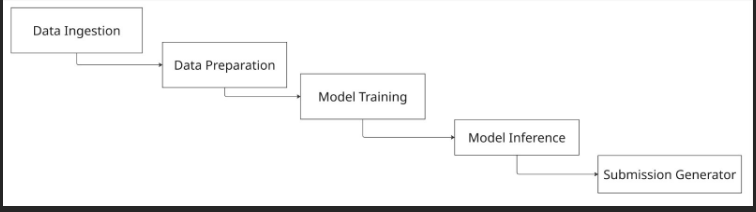
\includegraphics[width=\textwidth]{src/image.png}
    \caption{Pipeline for Predictive Model Development}
\end{figure}
    
\subsection*{Data Ingestion}

First, raw data is loaded. The competition provides four essential files to develop the predictive model:

\begin{description}
  \item[Train.csv] Training dataset containing the features necessary for the model to learn the underlying patterns.
  
  \item[Test.csv] Evaluation dataset where you will apply your trained model to generate predictions. Similar to the training set but without including the correct answers.
  
  \item[sample\_submission.csv] Template that specifies the exact format required to submit your final predictions to the competition platform, ensuring compatibility with the evaluation system.
  
  \item[train\_labels.csv] Contains the target answers that the model must learn to predict. This file includes the session identifier (session\_id), the corresponding question, and a binary indicator that shows whether the question was answered correctly or not.
\end{description}

This data structure, which separates features from labels, is designed to facilitate the development of a binary classification model that can effectively predict whether an answer will be correct or incorrect.

\subsection*{Data Preparation}

Once the raw data is loaded, the first step is to clean it to retain only the elements relevant for modeling, in addition to extracting relevant information that is not explicitly available. The goal is to extract features that are likely to correlate with student performance and reflect behavioral patterns in the game data.

\subsection*{Model Training}

Once the data is prepared, a machine learning model is selected for training. For this competition, a tree-based model is used, such as RandomForest, GradientBoostedTrees, CART, or DistributedGradientBoostedTrees, as they work well with structured data and effectively manage numerical and categorical variables. Additionally, they are ideal for capturing non-linear relationships in the dataset.

\subsection*{Model Inference}

Once the model is trained, inference is performed on the test set to evaluate its predictive accuracy. Multiple models can be tested to compare their performance and determine which offers the most accurate results.

\subsection*{Submission Generator}

Formatting predictions in the required format
and deploying to LLM Kaggle.

\subsection*{Systems Engineering Principles}

\begin{description}
  \item[Modularity:] The system was divided into independent components, each with a specific responsibility. In our case, modules were separated for data ingestion, cleaning and processing, feature engineering, model training, evaluation, and prediction.
  
  \item[Reusability:] Thanks to modularity, components can be reused without the need to modify the entire system. For example, if you want to train the model with another algorithm, it is not necessary to change the data ingestion module, and adjustments in processing would be minimal or none, depending on the requirements of the new model.
  
  \item[Scalability:] The system was designed to scale horizontally, allowing it to process larger volumes of data without affecting its structure. If more event records or new sessions are received in the future, the current components can adapt without redesigning the entire system.
\end{description}

\section{Addressing Sensitivity and Chaos}
In this section, we address the sensitive variables and chaotic factors identified during the system analysis in Workshop 1. The student’s performance in this context is modeled based on their interactions with the educational game. Multiple sources of variability were identified, including unpredictable user behavior, variable initial conditions, and random in-game events.

In terms of user behavior, we observed fast or erratic clicks, irregular mouse movements, and non-linear navigation paths. Regarding initial conditions, factors such as emotional state, motivation level, and familiarity with the game can significantly affect user interaction. Random events may include variations in question difficulty or game elements that introduce noise into the dataset.

The mitigation strategies implemented to address these challenges include:

\begin{enumerate}
    \item \textbf{Data Normalization and Preprocessing:}
    \begin{itemize}
        \item Elimination of erroneous and duplicate clicks.
        \item Standardization of \texttt{x,y} coordinate space.
        \item Extraction of temporal features.
    \end{itemize}
    
    \item \textbf{Use of TensorFlow Decision Forests (TF-DF):} \\
    TF-DF is robust to noisy data and can handle both categorical and numerical features without requiring additional encoding. The ensemble nature of decision forests enables the model to capture non-linear and complex relationships among variables, thus improving generalization capabilities.

    \item \textbf{Monitoring of Unanticipated Conditions:} \\
    Implementation of observation routines to detect unusual patterns or anomalies in the interaction data.
\end{enumerate}

\section{Technical Stack and Implementation Sketch}

The following tools will be used to build and train the model:

\subsection*{Programming Language}
\begin{itemize}
  \item \textbf{Python:} Main language due to its ease of use and its broad ecosystem for data science and machine learning.
\end{itemize}

\subsection*{Libraries and Frameworks}
\begin{itemize}
  \item \textbf{NumPy and Pandas:} For data manipulation, cleaning, and processing.
  \item \textbf{LightGBM or XGBoost:} For creating tree-based models, highly efficient for structured data.
  \item \textbf{Matplotlib and Seaborn:} For visualization and exploratory data analysis.
  \item \textbf{TensorFlow Decision Forests (optional):} For experimenting with advanced tree models within the TensorFlow environment.
\end{itemize}

\subsection*{Environment and Tools}
\begin{itemize}
  \item \textbf{Jupyter Notebooks:} For implementation, experimentation, and model documentation.
  \item \textbf{Git and GitHub:} For version control and collaborative work.
  \item \textbf{Kaggle Notebooks:} For testing and final submission of the model on the official competition platform.
\end{itemize}

\end{document}
